% Source: AESP_466_ClassWork/Supplements/Notes/latex/1.3/1.3_extended.tex
% Description: Simple pendulum with inertial Frame 1 (slate) and body Frame M (blue) attached to the mass.

\documentclass[border=4pt]{standalone}
\usepackage{amsmath,amssymb}
\usepackage{graphicx}
\usepackage{tikz}
\usepackage{xcolor}
\usetikzlibrary{arrows.meta, calc, patterns, angles, quotes, decorations.pathmorphing}

\definecolor{Garnet}{HTML}{73000A}
\definecolor{USC_Rose}{HTML}{CC2E40}
\definecolor{USC_Blue}{HTML}{466A9F}
\definecolor{USC_Slate}{HTML}{1F414D}
\definecolor{USC_Olive}{HTML}{65780B}
\definecolor{USC_Lime}{HTML}{CED318}
\definecolor{USC_Gold}{HTML}{A49137}
\definecolor{USC_Black90}{HTML}{565656}
\definecolor{USC_Black10}{HTML}{ECECEC}

\begin{document}
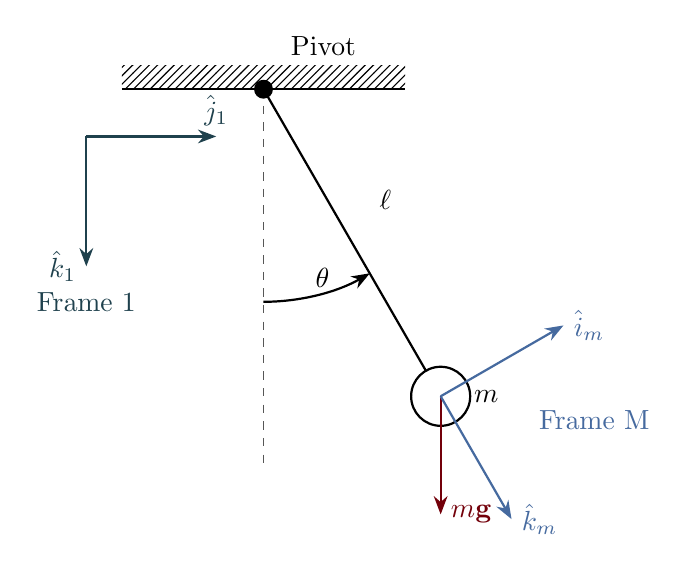
\begin{tikzpicture}[scale=1.5, >=Stealth]
    % Ceiling / Support
    \fill[pattern=north east lines] (-1.2,0) rectangle (1.2,0.2);
    \draw[thick] (-1.2,0) -- (1.2,0);

    % Vertical Reference Line
    \draw[dashed, USC_Black90] (0,0) -- (0,-3.2);

    % Rod
    \draw[thick] (0,0) -- (1.5,-2.6);

    % Pivot Point
    \fill[black] (0,0) circle (0.08);
    \node[above right] at (0.15,0.2) {Pivot};

    % Mass (Circle with white fill)
    \filldraw[fill=white, thick] (1.5,-2.6) circle (0.25);
    \node[right=0.3cm] at (1.5,-2.6) {$m$};

    % Angle Theta
    \draw[->, thick] (0,-1.8) arc (-90:-60:1.8);
    \node at (0.5,-1.6) {$\theta$};

    % Length label
    \node[above right] at (0.9,-1.1) {$\ell$};

    % Gravity arrow
    \draw[->, thick, Garnet] (1.5,-2.6) -- (1.5,-3.6) node[right] {$m\mathbf{g}$};

    % Inertial Frame axes (offset to left, below ceiling)
    \draw[->, thick, USC_Slate] (-1.5,-0.4) -- (-1.5,-1.5) node[left] {$\hat{k}_1$};
    \draw[->, thick, USC_Slate] (-1.5,-0.4) -- (-0.4,-0.4) node[above] {$\hat{j}_1$};
    \node[USC_Slate] at (-1.5,-1.8) {Frame 1};

    % Body Frame axes (at mass)
    \draw[->, thick, USC_Blue] (1.5,-2.6) -- (2.1,-3.64) node[right] {$\hat{k}_m$};
    \draw[->, thick, USC_Blue] (1.5,-2.6) -- (2.54,-2.0) node[right] {$\hat{i}_m$};
    \node[USC_Blue] at (2.8,-2.8) {Frame M};
\end{tikzpicture}
\end{document}
